\thesischapterexordium
\section{脑电的产生与现状}
脑电的先驱英国人Richard Caton在1875-1887年间先后开展动物研究\citing{haas2003hans},他把两个单极电极放在动物大脑的左右皮层或把一个电极放在皮层灰质另一个电极放在颅骨表面记录到了电流。他发现电流随着睡眠增强且呈现出与心跳、呼吸节律无关的变化,这些电流易受到缺氧或麻醉的影响,最终随着动物的死亡消失。基于Richard Caton的工作,德国人Hans Berger在1924年对一位17岁男孩进行外科手术时
第一次记录到了人类脑电,经过五年的反复推敲,最终于1929年发表题为Über das Elektrenkephalogramm des Menschen (人类的脑电) \citing{berger_uber_1929,millett2001hans,la1999history}的文章,他声称第一次从人类头皮表面记录到脑电活动,一段早期记录的脑电
波如图\ref{1:wave}所示。他在文中也首次描述了脑电的$\alpha$波(最早被称为Berger波)和$\beta$波,指出脑电会随着注意和情感效应而变化,特别是脑电波特征在癫痫等脑疾病中有明显变化。Berger在1924-1929年间重复脑电实验的过程中就认识到参考电极选择可能对脑电记录有影响并初步指出脑电波的不同节律特点。
\begin{figure}[!h]
	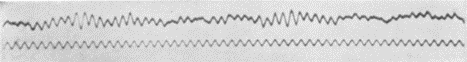
\includegraphics[width=13cm]{pic/xulun/EEGwave.png}
	\caption{Berger记录的第一条脑电波,引自文献\citing{berger_uber_1929}。}
	\label{1:wave}
\end{figure}

今天人们对脑电的认识更加清楚。如图\ref{1:record}A所示,脑电来自大量神经元同步放电活动的突触后电位总和,这种电位总和被头表电极和参考电极检测到经差分记录放大得到,反映了神经元的节律振荡\citing{niedermeyer_electroencephalography_2005}。图中的$A^{\prime\prime}$和$B^{\prime\prime}$分别是脑电记录的活跃电极和参考电极。参考电极的不唯一性和较低的空间分辨率成为脑电的两个主要劣势\citing{pascual-marqui_low_1994,pascual-marqui_r_d_and_lehamann_d_topographic_1993,rd_pascual-marqui_review_1999,teplan_fundamentals_2002}。自脑电产生以来,人们从未停止过对参考电极选择的研究。根据脑电的时域信号的幅度和波的快慢频率变化,人们在$\alpha$和$\beta$节律的基础上又将脑电分为如图\ref{1:record}B中五种不同类型的波,包括<4Hz的$\delta$节律、4-7Hz的$\theta$节律、8-12Hz的$\alpha$节律、15-30Hz的$\beta$节律和>31Hz的$\gamma$节律,称具有不同节律的频率范围为不同的频带。这些节律随着频率增加大致呈现幅度下降的趋势,与大脑的认知状态、神经功能的生长发育成熟或老化息息相关。当前实验室和临床中常用被试对某种刺激产生的事件诱发脑电研究被试的认知加工过程,或对静息态自发脑电活动进行定量谱分析,用以诊断癫痫\citing{tatum2014handbook}、睡眠紊乱、昏迷、中风、肿瘤和表征麻醉程度、脑死亡等\citing{chernecky2012laboratory}。脑电也在多模态融合、脑机接口、人机交互等工程领域得到广泛应用。
\begin{figure}[!h]
	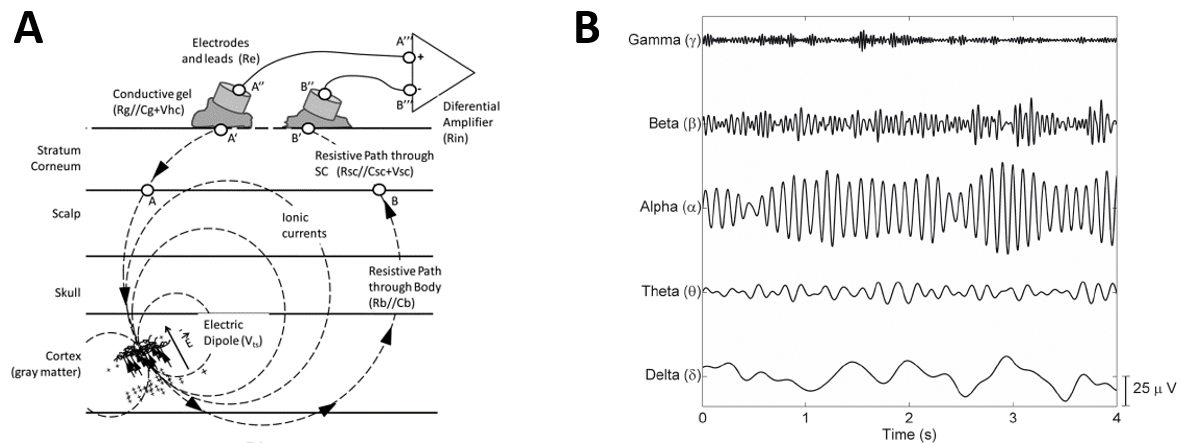
\includegraphics[width=15cm]{pic/xulun/record.png}
	\caption{A:脑电产生的偶极子、电流与差分记录,引自文献\citing{lopez2014dry},B:脑电的不同节律波形特点,引自文献\citing{campisi2012eeg}。}
	\label{1:record}
\end{figure}


\section{定量脑电定义}
定量脑电是相对于视觉分析脑电的波形特点如节律快慢、纺锤波有无、痫样放电等类似的定性分析而言的。视觉定性分析容易受到经验和专业知识的影响,促使人们提出更客观的分析方法。1932年,Dietsch的论文\cite{Dietsch1932}首次使用傅里叶变换分析七例头表脑电,这是定量脑电的开始
\citing{Kaiser2005}。19世纪80年代,美国纽约大学的E. Roy John在论文\cite{john1977neurometrics,john1980developmental}中提出定量脑电的概念,定量脑电是基于健康被试静息态脑电谱常模特征的诊断方法,这种谱常模可由脑电谱特征进行z分数标准化调整关于年龄因素的均值和偏差得到。z分数标准化\citing{glantz1990primer}公式为
\begin{equation}
z=\frac{x-\mu}{\sigma}
\end{equation}
这里的$x$可以是任意脑电谱特征,$\mu$和$\sigma$分别是该特征关于被试群体年龄因素的均值和标准偏差。基于谱常模,定量脑电的诊断方法包括谱常模特征提取和预测诊断等。定量脑电在神经反馈和临床诊断中得到广泛应用\citing{budzynski2009introduction,simkin2014quantitative}。

本论文中的定量脑电仅指传统意义上基于静息态脑电谱特征面向诊断应用的方法,相似的描述也表述在著作\cite{kropotov2010quantitative,evans1999introduction,nuwer1988quantitative}中。更广义地,采用数学和统计学方法估计那些视觉难以量化的特征都属于定量脑电分析,
书籍\cite{tong2009quantitative,majumdar2017brief}中描述了更广义的定量脑电分析方法。

\section{定量脑电研究方法}
随着信号采集、计算机和信号分析等技术的进展,脑电研究方法如图\ref{1:evol}左经历四个阶段:早期基于拍照成像的视觉分析,对纸质打印
脑电波进行统计分析、基于磁盘存储的编程分析和基于云存储的高性能计算分析\citing{vogelstein2016cloud}。脑电分析方法如图\ref{1:evol}右分为:可能影响其他分析方法的参考标准化和去伪差、按空间分为头表电极的多通道信号分析和溯源\citing{rd_pascual-marqui_review_1999}到源空间的分析;按角度分为脑电波时域波形幅度分析、微状态\citing{khanna_microstates_2015}等空间模式分析和通过傅里叶变换对信号的时不变特征进行频域谱分析;根据是否关注信号间的联系又分为谱分析和基于图论的脑连接脑网络分析;按照信号分析的复杂程度,可分为基于高斯稳态的线性分析和考虑复杂度、更高阶谱、混沌动力学、熵等非稳态非随机的非线性分析;最后根据应用并借助于机器学习方法,可分为脑电谱常模的回归和对脑状态脑疾病的分类预测等。
\begin{figure}[!h]
	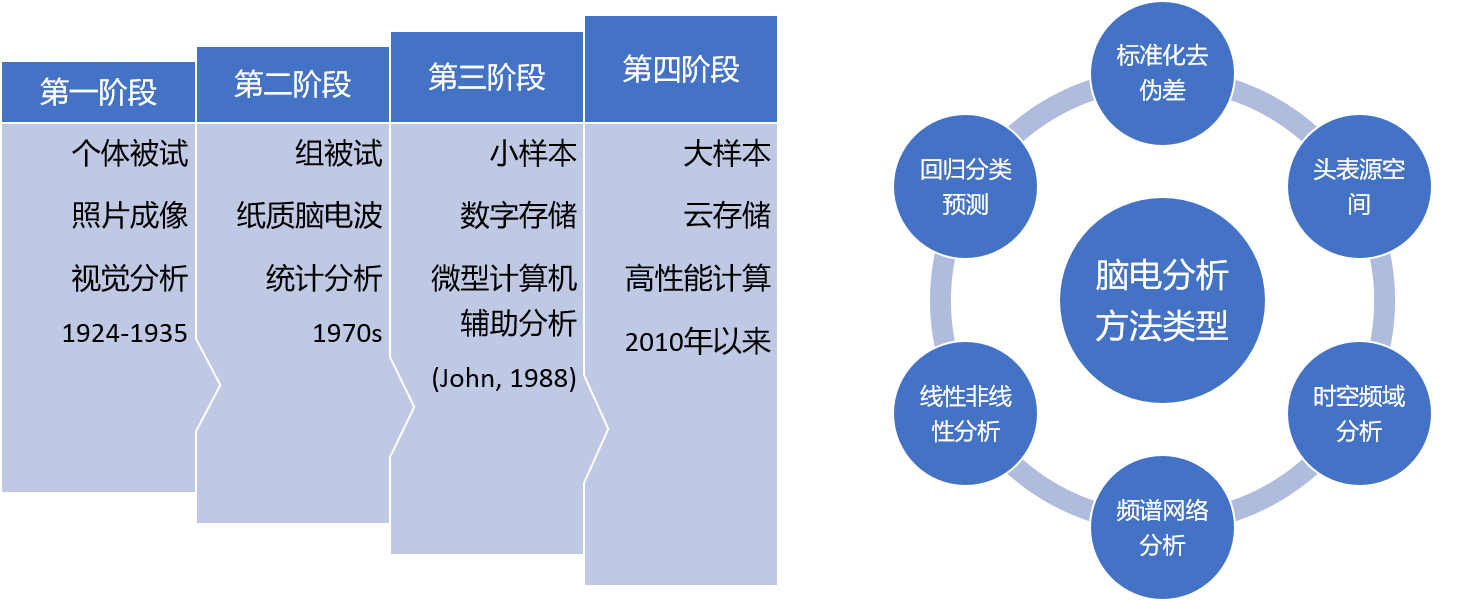
\includegraphics[width=15cm]{pic/xulun/evolution.png}
	\caption{脑电研究方法进展与类型。}
	\label{1:evol}
\end{figure}

但参考选择是进行脑电分析的基础和关键\citing{luck2014introduction},参考选择不规范是影响定量脑电分析的首要问题。定量脑电的定义表明定量脑电与基于谱数据选择、谱常模估计和谱特征提取紧密相关。本论文把参考与谱分析有关的技术作为定量脑电的重点研究内容。

\subsection{参考问题}
图\ref{1:record}A表示脑电信号的产生记录过程,脑电记录是活跃电极和参考电极的信号经差分放大记录得到的。脑电实际上是活跃电极信号减去参考电极信号得到的电势差\citing{teplan_fundamentals_2002}。根据电荷、偶极子及电场理论,测量电势的最优物理参考是距离测量带电荷无穷远处的位点,该位点具有零电势
是稳定的中立参考,被称为无穷远参考(Infinity Reference)。自脑电产生以来,人们一直进行不间断的尝试希望找到接近于理论无穷远参考的位点。如
今可供选择的参考种类繁多,图\ref{1:ref}列举了连接耳参考\citing{garneski_t_m_and_steelman_h_f_equalizing_1958}(Linked Mastoids
,LM)、平均参考\citing{offner_eeg_1950,goldman_clinical_1950}(Average Reference,AR)、左耳、右耳、偏侧耳(Ipsilateral ear)、头
表电极Cz、横向双极参考和纵向双极参考等。从\ref{1:ref}中可以看出,不同参考记录时的头表电位地形图相同但波形截然不同。这是因为参考的作用是连续记录中从所有活跃电极减去一维时变信号。尽管不同参考下活跃电极处的记录是相同大脑神经源活动经脑脊液、颅骨、头皮等传播到活跃电极处衰减叠加的信号,但不同参考意味着脑电差分记录中减去的信号不同。现有多种可供选择的参考造成参考使用不一致的问题,我们难以对不同参考的脑电分析结果进行对比。参考选择不规范以及由此产生的争论被称为参考电极问题\citing{yao_which_2019,hagemann_d_quest_2001,nunez_p_l_eeg_1997}。
\begin{figure}[!h]
	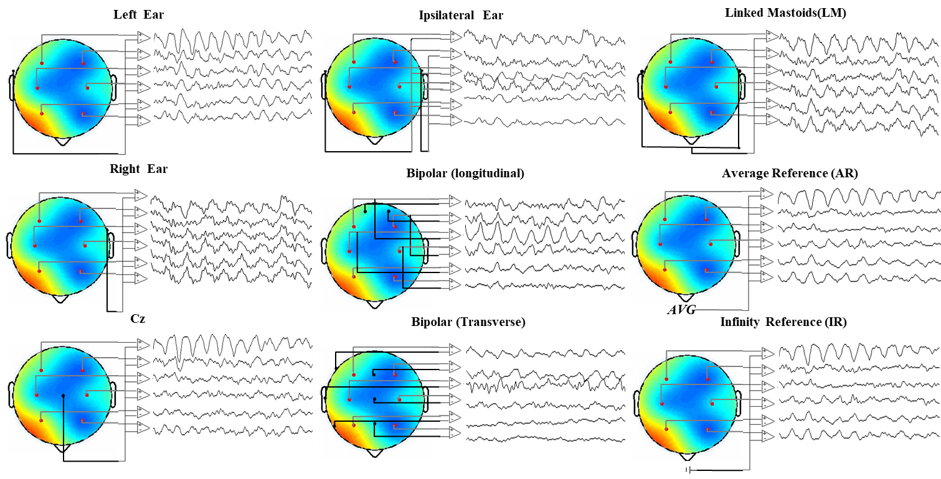
\includegraphics[width=15cm]{pic/xulun/EEGref.png}
	\caption{不统一的参考电极选择。左列为常用的在线记录参考,中间列为双极参考,右列为重参考。}
	\label{1:ref}
\end{figure}

\subsubsection{参考的类型}
脑电参考按照参考的步骤可分为在线记录参考和重参考\citing{hu_how_2018}。在线记录参考是脑电数据采集中主观选择的位于某一个空间位置的电极,一般由脑电采集设备生产商确定,常见的参考电极有FCz、Cz等。重参考是对获取的脑电记录进行离线分析时重新选择的参考,可能是将脑电记录中的某电极指定为参考电极,通常是对脑电记录进行电极间的线性结合得到的虚拟数字参考信号,常见的有连接耳参考、平均参考等。按照参考信号的唯一性可将脑电参考分为单极参考和双极参考等。单极参考是瞬时条件下从所有活跃电极减去相同的常数。双极参考在瞬时条件下从活跃电极上减去的常数不唯一,存在两个或更多。无穷远参考是一种单极参考。双极参考多数是横向或纵向顺次地将前一个电极作为后一个电极的参考,此时记录到局部相邻电极的相对电位。双极参考得到的脑电记录近似于脑电电位的一阶导,大多与头表的水平电流密度有关,是不同于单极参考下脑电电位的物理度量。偏侧耳参考是将一侧头表的电极参考到同侧的耳垂处的电极以消除左右半球的不对称性,这种双极参考记录增加了电极间差异的不确定性。单极参考是脑电参考的主要占优类型。本论文主要研究的是单极参考,可能是在线记录参考或重参考。

\subsubsection{参考选择}
在早期发现人类头表脑电的过程中,Berger仅将两个电极放在病人去除部分颅骨的皮层上或者健康被试的前额和枕叶,这是最早的参考选择。后来,人们相继基于不同假设提出不同的参考。因为与头皮较好的接触,Cz常被作为在线记录参考;根据左右耳垂电位均值为零的假设,连接耳也被广泛采用\citing{faux_preservation_1990,garneski_t_m_and_steelman_h_f_equalizing_1958};\cite{kulaichev_optimal_2016}一文最近还研究放在下巴、颈部、背部、鼻子等身体表面的参考电极接近无穷远参考的可能性。然而这些假设都不奏效,因为人体表面并不存在不活跃的零电位点,远离头表的体表电极还会采集到心电、肌电等伪差信号,置于体外的参考电极会引入环境噪声干扰,它们都与理论最优的无穷远参考相差甚远。

一种基于更多物理学假设的参考是平均参考。近似头表为封闭的球面,等效内部的神经源为偶极子活动,当偶极子在匀质导体内各向同性地传播,容积导体表面的电位积分为零,当头表被足够多的电极尽可能宽广覆盖并均匀分布采样,电极上电位的均值接近于零,所有电极上电位的均值可作为对无穷远参考的近似\citing{bertrand_theoretical_1985,nunez_p_l_eeg_1997,nunez_electric_2006}。从脑电记录减去所有电
极记录的均值后所有电极信号的均值为零,平均参考似乎具有接近实际的物理假设。近年来,D. Yao提出基于等效源技术和三层球头模型利用等
效源把任意脑电记录的非零参考转换为接近无穷远处参考的零参考(Reference Electrode Standardization Technique, REST)\citing{yao_method_2001}。

已有不少研究通过仿真或分析特定刺激的诱发电位研究参考选择的差异。但参考是一个数据转换过程。多种可选的参考方法都是给定某种参考的脑电记录对逼近无穷远参考脑电电位的统计学估计量。如果把不同的参考理解为给定实际脑电数据的多种备选统计模型,参考的选择就是统计学中的模型选择问题\citing{ando2010bayesian}。好的模型会平衡拟合的好坏和模型自身的复杂程度,拟合的好坏可以用似然函数来衡量,模型的简单复杂程度可以用自由度来表示。常用的模型选择准则包括Akaike信息准则\citing{akaike1998information}、Bayesian信息准则\citing{Schwarz1978}、广义交叉验证准则\citing{konishi_information_2008}、分步回归\citing{hocking1976biometrics,
draper1998applied}等。对多种参考进行模型选择分析有可能找到参考的理论差异和模型优劣证据。

\subsubsection{参考对脑电分析的影响}
D. Yao等对11例实际数据采用不同参考,发现低频和高频$\alpha$的头表空间谱地形图分布易受到参考的影响\citing{yao_d_comparative_2005}。L. Marzetti等仿真发现不当参考会对电极间的虚部相干造成失真,影响神经源间交互作用分析\citing{marzetti_l_use_2007}。仿真和奇数球范式
的诱发脑电数据分析说明不同参考对脑电数据的质量中心有较大影响\citing{qin2017comparative}。Q. Liu等仿真发现使用不当参考会造成脑电波形
失真\citing{liu_q_estimating_2015}。参考选择也被发现对相位滞后指数有较大影响\citing{thatcher2004eeg,nunez_p_l_eeg_1997}。Y. Qin等分析15例静息态闭眼脑电并结合仿真分析认为参考对不同频带下功率谱地形图分布、谱的幅度加权中心、相干估计、头表默认网络构建都有影响,证明频域分析的参考依赖效应\citing{qin_comparative_2010}。F. Chella等通过仿真和分析10例静息态睁眼脑电发现参考会对$\alpha$-$\beta$双相干模式带来较大失真\citing{chella_f_non-linear_2017},还发现网络连接空间模式、图分析的网络特征如节点度、局部效率等受到参考的影响\citing{chella_impact_2016}。这些结果说明参考的不规范使用会造成脑电波形、谱分析、网络分析等较大失真。因为定量脑电是谱分析、谱特征基于的方法,参考选择是进行定量脑电研究的首要问题。

\subsection{谱分析技术}
脑电是神经元的同步放电形成的,自然脑电信号中含有覆盖一定频带范围的有节律活动\citing{niedermeyer_electroencephalography_2005,buzsaki2006rhythms}。作为定量脑电分析的主要内容,谱分析用以量化脑电的不同节律振荡
。在Berger第一份关于$\alpha$、$\beta$波的报道中,他相信不同节律波反映不同大脑状态。如今已有大量的研究表明脑电谱与人类行为、认知状态、精神疾病之间有显著联系。根据不同的频带特性,脑电频带划分为$\delta$(1-3Hz)、$\theta$(4-7Hz)、$\alpha$(8-12Hz)、$\beta$(15-30Hz)和$\gamma$(31-100Hz)。尽管脑电频带的划分不尽相同,但小于1Hz的微小差异不会有太大影响\citing{nuwer1999ifcn}。一般低频活动反映潜意识的状态,主要在深度睡眠和困倦时占优,高频活动主要和警醒、活跃或更高级认知功能\citing{jensen2007human,sanei2013eeg}有关。

谱分析的步骤是首先通过傅里叶变换将脑电的时间序列信号从时域的幅度变化转换为频域单位时间内振荡的次数,再通过谱估计得到对应每个频率下的能量\citing{kay1999modern,stoica2005spectral}。谱分析的方法包括如周期图法、Welch法、Multitaper法\citing{thomson1982spectrum}等非参数估计和如自回归模型等参数估计。谱估计允许我们分析每个频带的绝对谱能量、相对谱能量和谱的地形图分布\citing{Li2019eeg}。定量脑电中我们将谱的特征与数据库的谱常模进行对比研究被试与正常值的偏差\citing{Kim2018}。除了多通道电极
的功率谱分析,我们还可以分析电极间的交叉谱和双谱、三阶谱等\citing{nikias1993signal}。交叉谱分析是进行头表或神经源空间频域连接
、网络分析的常见步骤。

\subsubsection{谱质量准则}
失真的谱不能反映出健康被试的真正脑电频域信息还作为离群值影响谱常模的估计甚至使最终提取出的谱特征与被试认知状态、疾病机制相差甚远。谱估计的质量不仅依赖于参考选择还可能受到脑电数据去伪迹程度的影响。脑电记录中与大脑神经活动无关的信号都是伪迹。电极较强的敏感性极易在测量信号中引入如表\ref{1:noise}中的生理伪迹\citing{brittenham1974recognition}如眼电、肌电、心电和出汗、呼吸、咀嚼等
过程有关的皮电,以及环境伪迹\citing{saunders1979artifacts}如头动或电极接触不良带来的漂移、接地不良引起的工频干扰、电极阻抗的
升高和电极导线的电磁干扰、噪音等。
\begin{table}[!h]
	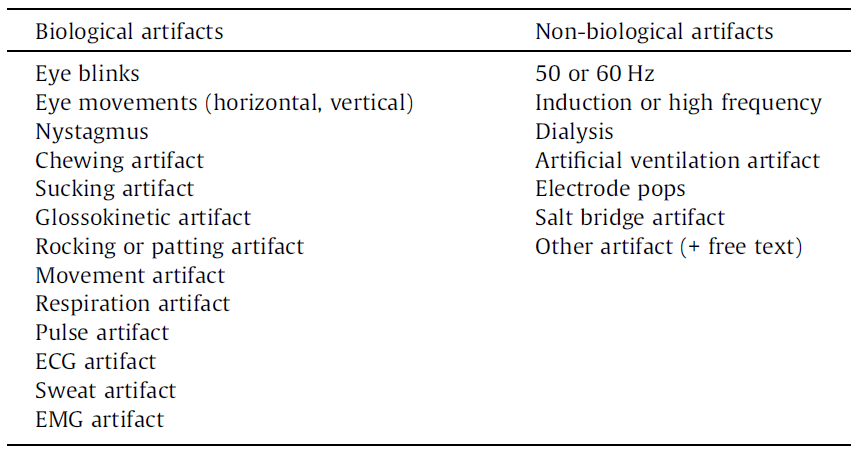
\includegraphics[width=12cm]{pic/xulun/EEGnoise.png}
	\caption{脑电信号伪迹,引自文献\citing{beniczky2017standardized}。}
	\label{1:noise}
\end{table}

谱质量与脑电数据质量、伪迹去除紧密相关。目前伪迹去除的研究已较为成熟。电生理专家或临床医生根据经验或参照国际临床电生理联盟推出的SCORE\citing{beniczky2017standardized}和脑电图伪迹手册\citing{lara2015rowan}手动去伪迹。这种方法容易受专家研究动机、疲惫程度、知识和经验等主观因素的影响且只适合小样本数据分析。相比,一种更加客观的分析是基于独立成分分析,假设不同成分的伪迹与脑电成分相互独立,采用独立成分分析\citing{delorme2007enhanced,jung2000removing}根据成分权重的地形图形状等来标注成分的类型\citing{pion2019iclabel}拒绝伪差成分。具有独立成分分析又能进行坏道挑选、滤波、参考变换、插值和回归的软件有EEGLAB\citing{delorme2004eeglab}、MARA\citing{winkler2011automatic}、FASTER\citing{nolan2010faster}、ADJUST\citing{mognon2011adjust}、SASICA\citing{chaumon2015practical}和Automagic\citing{pedroni2019automagic}等。定量脑电中建立谱常模通常是基于大样本的谱数据,使用独立成分分析进行预处理成为首选。

一个被忽视的问题是如何控制去伪迹的程度。独立成分分析等方法可能在去噪的同时丢失掉与脑活动有关的信号,这是因为成分间的统计独立假设并不能有效区分脑活动和各种伪迹,比如权重较小、地形图不明显像偶极子活动的成分也可能是脑电信号。去除成分可能丢失与脑活动有关的成分,对坏道插值可能引入共线性等。当前脑电预处理主要关注时域波形特点,缺乏有效的质量控制。预处理后似乎正常的脑电波形的频谱信息可能遭到破坏,可能出现谱同构的问题。发展一种能表征谱质量对脑电和谱数据质量筛选的准则十分重要。

\subsubsection{谱常模回归}
正常被试的脑电随着年龄变化的谱常模曲线可作为大脑正常的生长规律曲线,是研究神经功能发育成熟以及老化过程中出现异常的重要参照标准。建立脑电谱常模是提取谱特征进行分类诊断的前提。主要方法是用回归揭示大样本脑电谱数据与年龄、频率等因素的关系。常见的回归模型包括线性回归、多项式回归、广义线性模型、逻辑回归、具有固定效应和随机效应的混合模型、非线性回归、非参数回归、鲁棒回归和局部移动回归等。

线性回归是采用普通的最小二乘法找到唯一的曲线或超平面使拟合数据与实际数据间残差的平方和最小。混合模型中具有固定非随机参数的自变量是固定效应,与群体有关但随个体变化的自变量是随机效应\citing{pinheiro2006mixed,demidenko2013mixed,gardiner2009fixed}。非参数回归没
有固定自变量,通常需要较大的样本量,如高斯过程回归(Kriging)和核回归等。高斯过程回归基于先验协方差的高斯过程进行插值,常用于空间分析中对随机空间场的个别点估计,是一种重要的空间插值方法\citing{williams1998prediction,wahba1990spline}。局部移动回归\citing{garimella2017simple,cleveland1988locally}是局部多项式回归和移动平均的推广,常见的方法是局部加权的散点图平滑\citing{cleveland1981lowess}(Local Weighted Scatterplot Smoothing, LOWESS)。分步回归能自动地在拟合回归模型中选择自变量,基于预定义的准则分步从因变量集中加减某个变量,包括正向选择、反向消除和双向消除自变量直到模型最终稳定。回归模型参数的估计方法有最小二乘、脊回归(Tikhonov正则化)、贝叶斯线性回归和迭代再加权最小二乘等。

\subsubsection{谱特征提取}
有效提取谱特征是应用定量脑电到认知加工机制研究、生物标记物识别、神经反馈和疾病诊断的关键。只有有效提取相关特征才能提高预测和诊断疾病的准确率。谱特征是神经振荡在脑电中的集中显现。傅里叶变换将脑电波分解为频率和幅度不同的正弦曲线,谱曲线反映周期振荡的节律信息在某个频带表现为谱峰。脑电节律由丘脑皮层系统大范围抑制过程的神经同步活动引起\citing{andersen1968physiological,Steriade1990}或神经元兴奋抑制
间的负反馈形成\citing{freeman1975mass}。大量研究表明周期振荡和生理、认知、行为和疾病状态有关,同时大脑中还存在随年龄、认知状态、任务
压力改变和生理过程有关的非周期振荡。非周期的振荡信息在谱中表现为随着频率增加而下降的曲线,这条曲线被称为1/f过程\citing{abry1995wavelets}或粉噪声(pink noise)。

谱特征提取的主要问题是具有不同共振频率的周期振荡在宽频带上相互叠加,周期振荡的谱总与非周期振荡的谱叠加。这要求只有先对谱曲线进行代表不同振荡的谱成分分离才能提取特征。周期振荡的特征有代表共振频率的谱峰频率位置、表示振荡强度的谱峰能量、代表振荡范围的带宽等。非周期振荡谱的主要特征是斜率和截距,前者与神经元群的兴奋抑制的共济效应有关\citing{gao2017inferring},后者可能与整个神经元群的集体放电
\citing{manning2009broadband,miller2012human}、fMRI的BOLD信号有关\citing{winawer2013asynchronous}。

\section{当前定量脑电方法存在的问题}
图\ref{1:qEEGnext}总结了当前定量脑电方法存在的问题以及可能取得的进展。主要问题是: 1.多样的数据格式有待统一到BIDS标准\citing{pernet2019eeg}以便于数据的存储和分享;2.存在参考选择问题,多种的参考方法需要规范起来,减少数据间因为参考带来的差异,便于数据存储和实验室间的比较研究;3.当前的脑电数据伪差去除主要是基于独立成分分析的方法,缺乏质量控制标准,缺乏一种对大样本谱数据进行质量控制的准则;4.存在某个地区的脑电谱常模但能否建立多国家或国家间通用谱常模并不清楚,国际通用的脑电谱常模便于进行大样本数据分析得到更加信服的结果并用于国际上某地区特殊群体的疾病诊断;5.当前只存在对谱曲线中$\alpha$节律和背景神经振荡的参数拟合方法,缺乏能有效分离常模谱成分及提取
特征的方法;6.谱常模主要是基于功率谱的单变量分析,并没有考虑神经源间的交互连接,有待从单变量功率谱扩展到多变量交叉谱或者相干网络;7.谱常模的特征提取、分类诊断是在欧式空间,我们可以借助于黎曼学习直接对交叉谱矩阵在黎曼流形上进行分析,采用更符合数据结构和空间特性的方法有助于识别出更准确的生物标记物。
\begin{figure}[!h]
	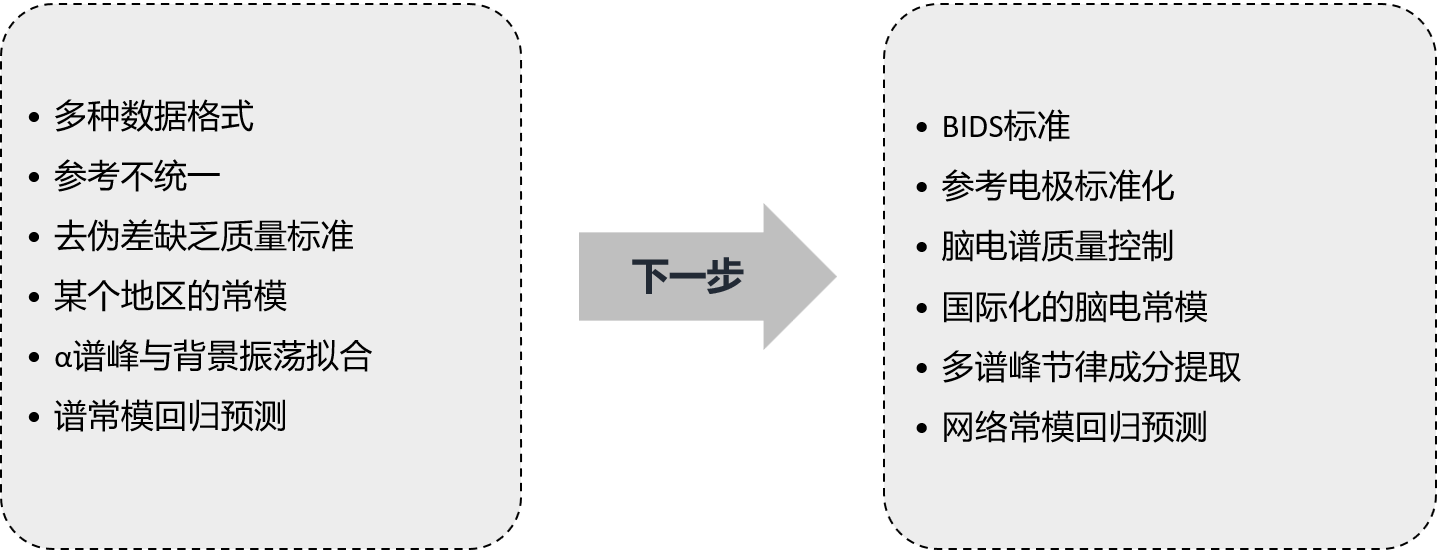
\includegraphics[width=12cm]{pic/xulun/qEEGnext.png}
	\caption{当前定量脑电方法可能取得的进展。}
	\label{1:qEEGnext}
\end{figure}

\section{本文拟解决的问题}
因为参考选择对脑电频谱分析有显著影响,定量脑电主要依赖于谱分析,本论文把参考选择和谱分析相关技术作为重点分两部分研究。第一部分,我们首先研究在实际数据采集的不同因素下,已有参考选择对逼近理论最优无穷远参考的效果,探究参考对不同物理因素的鲁棒性;然后利用统计学习的方法找到参考选择的模型指数证据;又分析不同参考间的关系,平均参考和零参考物理假设的数学意义,建立参考家族及其属性。第二部分,我们首先提出对脑电数据的谱质量初步筛选的准则;再探讨不同国家被试群体之间是否存在一致的脑电谱常模演化曲线的问题试图对多国家脑电数据估计出谱常
模,最后发展谱成分分离和特征提取的合理模型。

\section{本文的主要贡献与创新}
本论文以定量脑电中的参考选择和谱分析技术为重点研究内容,主要创新点与贡献如下:

1. 从参考的物理学假设出发,我们首次全面系统地分析参考模态和电极配置等多种因素对脑电电位准确性的影响,这些因素包括:从稀疏到致密的11种覆盖从临床到科研作者所能见到的电极数目、2种电极分布即按电极距离如10-20/10/05分布和按多边形剖分的测地网GSN分布、不同的头模型(三层同心球头模型和基于结构磁共振数据的真实头模型)、容积传导模型的扰动、神经源偶极子的位置方向、头表电极的位置以及电极噪声等。主要贡献是发现平均参考并不随电极数目的增多而改善,依赖于电极覆盖区域和偶极子活动方向,零参考对头模型的准确性不敏感。这与一直以来对二者基于物理学假设的直观认识不同,使我们对不同因素下参考的性能区别有了新的认识。

2. 我们首次提出广义线性参考模型,利用惩罚的最大似然估计发现平均参考和零参考服从参考的通解,二者的区别在于先验协方差的差异,最后利用广义交叉验证、Akaike和Bayesian信息准则对二者基于仿真和实际数据进行选择,我们发现零参考具有比平均参考更优的模型准则。 我们还首次发现广义交叉验证是实际零参考应用中选择去噪参数的最优准则,提出在实际的零参考应用中可采用被试群体的平均传递矩阵代替被试个体传递矩阵。 主要贡献是我们首次提出参考问题的统一贝叶斯架构,认为平均参考是基于多通道脑电信号间相互独立的假设而零参考引入容积传导效应的先验假设,第一次从模型选择的角度找到零参考优于平均参考的证据。

3. 我们研究更多单极参考发现它们都具有满秩减一的特性。 将该特性推广到无穷远参考下的传递矩阵并通过满秩减一型矩阵逆引理,我们首次证明零参考和平均参考、连接耳参考及其他在线记录参考一样都是单极参考。基于零参考和平均参考的物理学假设,我们首次从约束线性回归的角度推导出零参考和平均参考,证明二者是在对应约束下的合理选择。 主要贡献是我们建立了单极参考家族,分析单极参考具有三个重要属性,分别是无记忆性,即单极参考之间相互独立可以任意变换,单极参考都具有满秩减一的属性,以及单极参考算子和单极参考下传递矩阵分别具有正交投影中心化(等于平均参考)和加权中心化的属性,证明零参考与其他参考的不同在于借助于容积传导效应进行加权中心化。

4. 我们首次发现脑电预处理过度可能导致多通道谱平行或谱同构的问题。基于共同主成分分析,我们提出衡量谱同构异质性的准则,用这种准则可以对谱质量进行初步筛选,避免构建常模中高度同构的数据。

5. 借助于三个国家基本覆盖生命周期的数据,我们使用线性混合效应模型首次研究了脑电常模构建是否依赖于国家或个体因素,基于非参数回归得到多国家脑电谱常模演化曲面。这是第一个试图建立国际化通用脑电谱常模的研究。

6. 我们发现脑电谱成分拟合的合理准则是对独立于频率服从复高斯分布的傅里叶系数进行最大Whittle似然估计,认为谱多个节律成分的分离问题是协方差丢失的不完全数据估计问题可以通过最大似然估计来求解。我们首次采用平滑和单调性约束的非参数拟合取得比参数拟合更优的效果,将提出的$\xi\pi$模型应用在颅内脑电数据集上进行谱成分分解并提取参数。基于高斯过程回归,我们建立了全脑空间在任意频率下的谱振荡地形图。

\section{本论文的结构安排}
本论文中研究的定量脑电是频谱分析和谱特征基于的方法。一直以来定量脑电存在参考选择不唯一、不规范的问题,已有研究表明参考选择对频谱分析有显著影响。我们在第一部分(第二至四章)中研究参考选择的物理因素、数理统计学证据、共同属性和联系,再在第二部分(第五至七章)探究与谱分析有关的技术,于第五章中提出基于谱结构的质量筛选准则,于第六章研究多个国家建立脑电谱常模的可能性,于第七章发展对脑电谱成分分解和谱特征提取的$\xi\pi$模型。前后两部分是并列关系,但第一部分在内容上更加深入全面,第二部分仅是对谱分析相关技术的初步探究。全文的结构安排如
下:
\begin{description}
	\item[第一章] 绪论。主要介绍脑电的产生、研究方法进展以及定量脑电定义和研究方法现状。特别是对关键词参考、谱分析相关技术等进行解释,为全文的研究作下背景知识铺垫,最后对全文的研究内容和结构安排做简单介绍。
	\item[第二章] 以参考模态和电极配置为重点研究多种物理因素对定量脑电电势的影响。
	\item[第三章] 提出脑电的广义参考模型,描述脑电无穷远参考的统一贝叶斯架构,对平均参考和零参考进行基于统计模型指数的选择。
	\item[第四章] 证明零参考是一种单极参考,利用平均参考和零参考的物理约束通过线性回归的方法推导出了平均参考和零参考,建立单极参考家族,推导单极参考的联系和共同属性。
	\item[第五章] 指出预处理中可能存在丢失脑电成分造成谱同构的问题,提出基于谱结构的数据质量筛选准则(PaLOS指数),并在三个不同的数据库以及多个预处理步骤中验证PaLOS指数的效果。
    \item[第六章] 分析多国家脑电数据中的国家、个体因素对构建谱常模的影响,并采用非参数回归构建多国家谱常模演化曲面。
	\item[第七章] 主要发展基于Whittle似然和非参数估计的谱节律成分提取算法$\xi\pi$模型,并分析大样本颅内脑电数据集,在完成谱成分分析和特征提取之后,我们基于高斯过程回归得到了任意频率全脑空间任意位置的谱地形图。
	\item[第八章] 总结全文工作的主要结果和创新点,梳理局部章节可能存在的不足,对需要完善的地方我们展望以后可能开展继续研究的出发点。
\end{description}